\section{Моделирование предметной области и разработка функциональных
требований}

{
\renewcommand{\mathbf}[1]{#1}
\subsection{Сенсоры}

Для получения информации об окружающей среде используются различные сенсоры.

\subsubsection{LIDAR}

\begin{figure}[h]
\centering
	\fbox{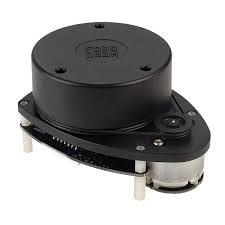
\includegraphics[width=9cm]{2d_lidar}}
\caption{2D LIDAR}
\end{figure}

Сенсор LIDAR выдаёт 2D снимок помещения -- облако точек в двумерной плоскости.
Используя облако точек, и зная позицию в которой снимок облака был совершён,
возможно реконструировать карту окружающего пространства на сетке. Если провести
отметить все клетки через которые прошёл луч за пустые, и отметить последнюю
клетку которую луч зацепил в качестве отмеченной, то получается 

\subsubsection{IMU}
Сенсор IMU (inertial measurement unit) даёт информацию об угловом и линейном
ускорении, что позволят определять текущее положение в пространстве.

\begin{figure}[h]
\centering
	\fbox{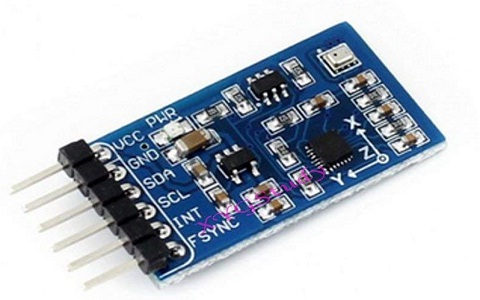
\includegraphics[width=9cm]{IMU}}
\caption{IMU}
\end{figure}

\subsubsection{GPS}
%\todo{По факту RTK может быть?}
Сенсор GPS выдаёт глобальную позицию в мировых координатах. Типичная точность
современных GPS-приёмников составляет 6-8 метров при хорошей видимости
спутников. 


% \subsection{Общие сведения и требования к работе программного средства}
%
% % \subsection{Описание функциональности программного средства}
% %
% % \todo{USECASE диаграмма}
% % \subsection{Спецификация функциональных требований}
%
% - Моделируем навигацию
% - Occupancy grid
% - Надо переместится в указанную точку на карте
% - Способ указывания точки на карте
%
% % \todo{ Если цель переместится в указанную точку, для этого надо построить
% % маршрут, чтобы построить маршрут нужна карта, чтобы построить карту используем
% % позицию и показания с сенсоров и метод SLAM }

\subsection{Разработка функциональных требований к проектируемому программному
средству}
% WATER
	Для успешной реализации системы мобильной навигации необходимо четко
	определить и описать функциональные требования, которые будут обеспечивать
	эффективность и точность работы системы. Эти требования являются основой для
	проектирования и разработки как аппаратной, так и программной части системы.
	В данном разделе мы рассмотрим ключевые аспекты, которые должны быть учтены
	при разработке функциональных требований для мобильной навигации, включая
	работу с картами, выполнение маршрутов и интеграцию различных сенсоров.

Система должна:
\begin{itemize}
	\item получать данные с сенсоров IMU, GPS, LIDAR;
	\item обрабатывать полученные данные и определять текущую позицию;
	\item строить карту окружающей среды;
	\item строить и выполнять маршут перемещаясь в указанную позицию;
	\item сохранять и загружать построенную карту между запусками;
\end{itemize}

\subsection{Разработка технических требований к программному средству}

Разрабатываемое программное решение должно обеспечивать корректное
функционирование при развёртывании на компьютерном модуле BananaPi CM4, или
на модуле со следующими техническими характеристиками:

\begin{itemize}
	\item оперативная память 4 Гбайт или более;
	\item amlogic A311D шести ядерный процессов с четырьмя Arm Cortex-A73
		ядрами, двумя Arm Cortex-A53 ядрами, или более быстродействующий
		процессор;
	\item доступный объём дискового пространства 5 Гбайт. %20mb на самом деле
\end{itemize}
